%Conclusion body
%Created SS 04-14

\section{Results}
\label{results}

\subsection{Second Sound Results}
\label{secondsoundresults}

To measure the velocity of second sound in He II, the propagation time of heat pulses in the superfluid is observed over a range of temperature.  First the displacement between the balometer and the heater (both fully submerged) was measured. Next, a heat pulse was sent from the heater which then propagated towards the balometer as second sound.  The duration between the triggering of the heat pulse and the pulse's signature recorded by the balometer was observed and recorded.  Multiple displacements and corresponding durations were recorded for various temperatures ranging from $1.6$ K to $2.2$ K (shown in Figure \ref{fig:secondsoundraw}). Second sound velocity goes to zero as the temperature approaches $T_{\lambda}$, after which the propagation of second sound can no longer be detected by the balometer.  


\begin{figure}[htbp]
\begin{center}
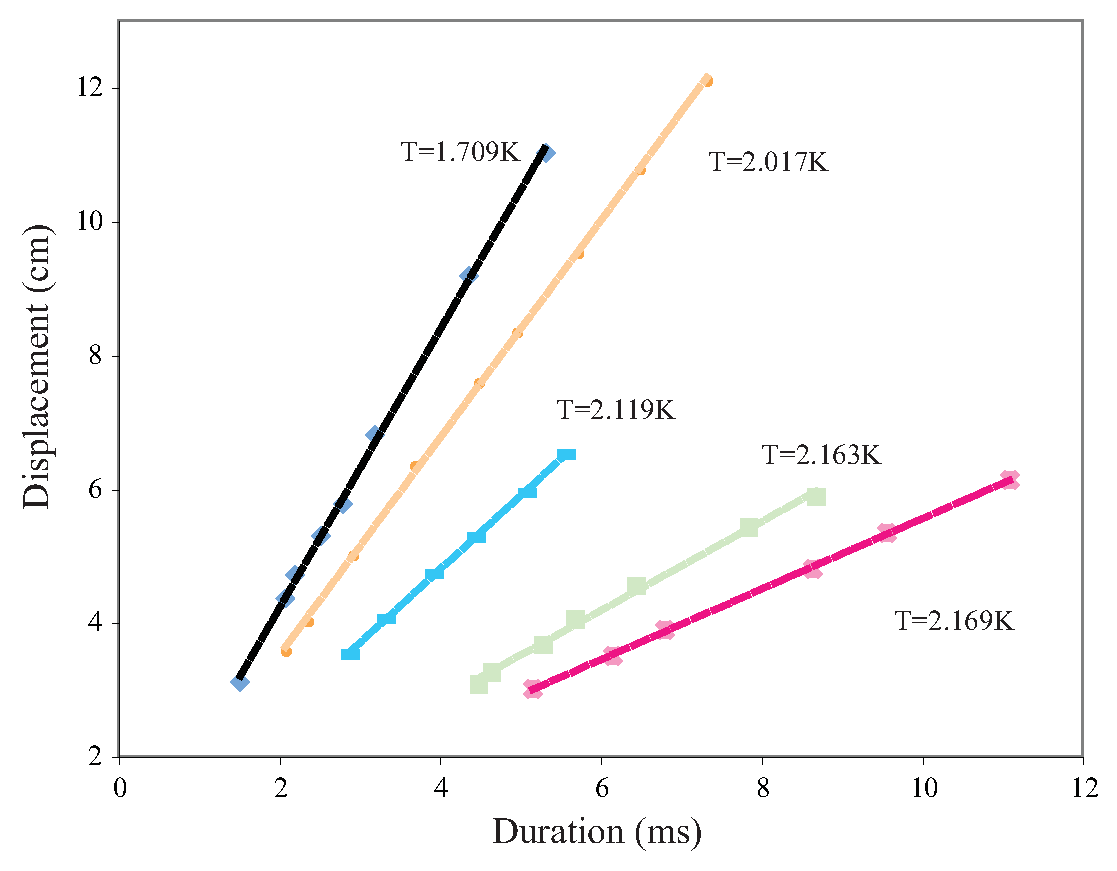
\includegraphics[height=70mm]{./figures/secondsoundraw.eps}
\caption{\small{A plot of the displacement of the thermometer from the heater verses the duration between the triggering of the heat pulse and the pulse's signature recorded by the thermometer for various temperatures in He II.}}
\label{fig:secondsoundraw}
\end{center}
\end{figure}


\subsection{Heat Capacity Results}\label{heatcapacityresults}

To measure heat capacity, we observe the effect of heat pulses sent to the cell on a germanium resistor which is thermally coupled to the cell.Beginning at a temperature of about $1.8$ K, $10$ ms heat pulses with a power of $98.8$ mW were sent to the cell.  These heat pulses caused the temperature of the cell to rise which consequently caused the resistance of the coupled germanium resistor to increase.  Because the current through the germanium resistor is constant ($1.00$ $\mu$A), a decrease in resistance causes a decrease in the potential difference across the resistor. The change in the potential difference due to consecutive heat pulses sent to the cell was measured while the Cu addendum was both filled and evacuated.  Figure \ref{fig:rawdata} shows portions of this data for both scenarios.  Over the course of the experimental run, the potential difference falls discretely due to the consecutive heat pulses in both cases, which corresponds to the incremental heating of the cell. While the heating of the Cu addendum by itself has a relatively uniform effect on the changes in potential for the entire observed temperature range, heating the filled addendum affects the changes in potential differently dependent upon whether the temperature of the cell is above or below $T_{\lambda}$.  This disparity is shown in Figure \ref{fig:rawdata}. 

\begin{figure}[htbp]
\begin{center}
\subfigure[Cu Addendum]{\label{fig:edge-a}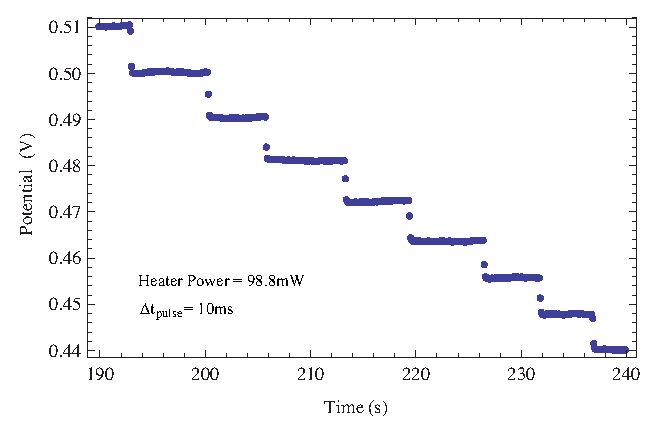
\includegraphics[height=52mm]{figures/rawcu.eps}}
\hspace{-1mm}
\vspace{-2mm}
\subfigure[He (II) and Cu Addendum near $T_{\lambda}$]{\label{fig:edge-b}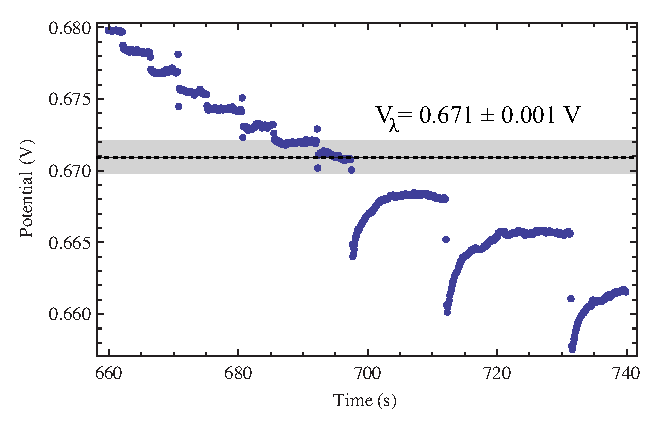
\includegraphics[height=52mm]{figures/rawhe.eps}}
\vspace{-2mm}
\caption{\small{Plots showing the change in the thermometer's potential difference due to heat pulses sent to (a) the evacuated addendum and (b) the addendum filled with He(II).  Each heat pulse is $10$ ms with a power of $98.8$ mW.  From this data we see that $T_{\lambda}$ occurs at $0.671 \pm 0.001$ V judging by the sudden change of the heat pulse's signature.}}
\label{fig:rawdata}
\end{center}
\end{figure}

Knowing the amount of energy deposited in the cell along with the change in temperature, we can calculate heat capacity of the evacuated Cu addendum and the Cu addendum filled with He.  To calculate the heat capacity of only the He, we will subtract the heat capacity of the evacuated addendum from the heat capacity of the filled addendum.  